% METODOLOGIA
\setlength{\fboxsep}{1cm}% Espaçamento interno do fbox
\fbox{% Cria um box ao redor do texto
    \parbox{\textwidth}{% Permite o controle de parágrafo dentro do fbox
        \setlength{\parindent}{1.5cm} % Define a identação dos parágrafos
        \fontsize{30}{36}\selectfont % Ajusta o tamanho da fonte e o espaçamento de linha
        \textbf{Metodologia}\\

\par{
    A integração de dados geológicos com modelos de IA é refinada pela sistematização proporcionada pela articulação de folhas de carta. Esta sistematização não só garante a consistência e precisão na organização dos dados, mas também otimiza o processo de alimentação dos modelos de IA. As folhas de carta servem como uma estrutura base que guia a coleta de dados, garantindo que cada informação geológica inserida no banco de dados PostgreSQL/PostGIS esteja bem organizada e pronta para análise.
}\\
\par{
    O uso dessa metodologia permite uma abordagem dinâmica e iterativa para a geração de mapas litológicos preditivos. Com a estruturação dos dados facilitada pelas folhas de carta, os modelos de IA podem ser aplicados de maneira mais eficiente, proporcionando análises preditivas mais precisas. A validação dessas predições por especialistas e a reincorporação de dados validados ao banco promovem um ciclo contínuo de aprimoramento, destacando a importância da articulação de folhas de carta não apenas para a automação, mas também para a evolução constante do projeto.
}\\

    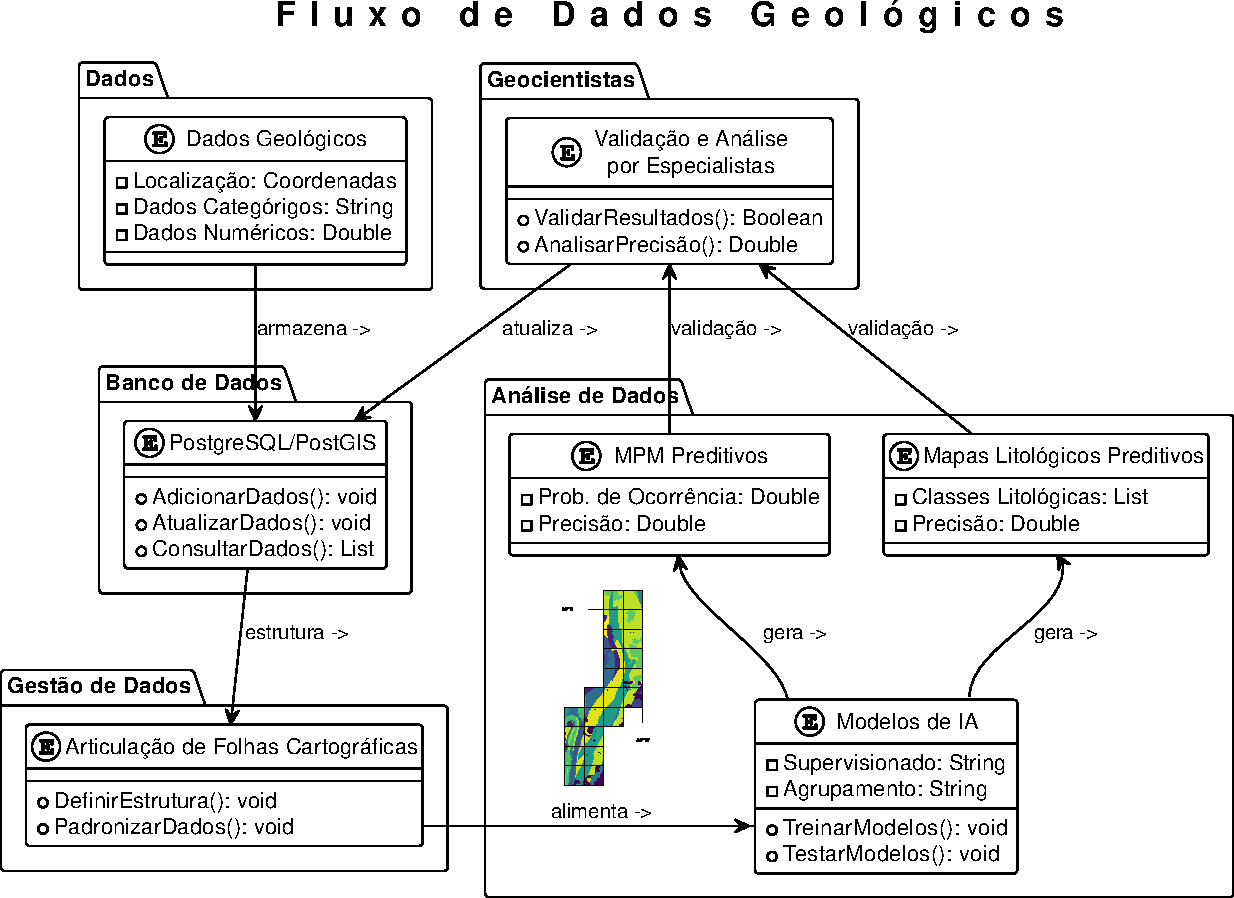
\includegraphics[width=0.9\textwidth]{imgs/PreditorTerraa.pdf}
    \captionof{figure}{\textbf{Diagrama simplificado do fluxo de dados entre as etapas de armazenamento, estruturação, análise e validação.}}

    \vspace{1.0cm}
    \justifying
    \setlength{\parindent}{1.5cm} % Define a identação dos parágrafos
    } % Fecha o parbox
} % Fecha o fbox
